\documentclass{beamer}
\usepackage{tabularx}
\usetheme{Copenhagen}

\begin{document}



\frame{ \frametitle{Introduction}
  Any educational program can be thought of as a sequence of tuples
   \[
     (\chi_i, t_i)
   \]
  which is an item scheduled at a time. An item could be a question or an
  informative content item. When placed in sequence, these form a schedule:
   \[
     X = \langle (\chi_1, t_1), (\chi_2, t_2), \ldots (\chi_n, t_n) \rangle.
   \]
  The present work seeks to answer the question: knowing the properties of
  these items, and having per-student information about the responses to
  these items at any point $i$, how should the remainder of the items be
  sequenced (or scheduled)?
}



\frame{ \frametitle{Novel Contributions}

  \begin{itemize} 

   \item The graph data structure to represent an assessment, whose nodes are
   items, and whose eduges represent dependencies;

   \item A modification to an existing assessment theory known as Item Response
   Theory, which now accounts for dependency relationships;
   
   \item A scheduler, or algorithm whose purpose was to determine what the
   questions should be given the item parameters and the students' response
   sets;

   \item An addendum to an existing theory of memory, forgetting, and practice,
   which could then be integrated into the scheduler to provide a
   fuller-featured system.

  \end{itemize} 

}



\frame{ \frametitle{Bloom's Taxonomy}

  \begin{itemize} 

    \item \textbf{Knowledge}. Recalling factual information.  \emph{What is a
    for-loop?}

    \item \textbf{Comprehension}. Assigning meaning to information.  \emph{What
    does the example for-loop output? (Give example.)}

    \item \textbf{Application}. Applying a rule to a specific instance.
    \emph{How can the update statement of the loop be changed to print only
    even numbers?}

    \item \textbf{Analysis}. Breaking information into parts and exploring
    relationships.  \emph{What would happen if the update statement decremented
    instead of incremented the counter?}

    \item \textbf{Evaluation}. Judging the use of knowledge or the validity of
    an argument.  \emph{Which is better for reading user input: a for-loop or a
    while-loop? Why?}

    \item \textbf{Synthesis}. Utilizing knowledge to create a new solution to
    satisfy a goal.  \emph{Write a for-loop to print only even numbers up to
    ten.}

  \end{itemize} 

}



\frame{ \frametitle{Item Response Theory}

  The motivation for Item Response Theory is to have a method of assessment
  which accounts for item difficulty, individual variance in student ability,
  the probability of guessing a question correctly, and the extent to which
  the item correlates with overall performance. 

}



\frame{ \frametitle{Item Response Theory}

  In Item Response Theory:

  \begin{itemize} 

   \item $\alpha$ is the item discrimination, or how well the item can
   distinguish students of varying trait ability;

   \item $\beta$ is the question difficulty, 

   \item $\gamma$ is the probability of guessing the answer correctly,

   \item and $\theta$ is the \emph{trait ability} of the student, or the
   student's particular ability to answer that question correctly.

  \end{itemize} 

}



\frame{ \frametitle{Item Response Theory}
 The Item Response Theory formula for calculating the probability that a student
 will answer a question given item parameters and student ability:
 \[
   p_i(\theta_s) = \gamma_i + \frac{1-\gamma_i}{1+e^{\alpha_i(\theta-\beta_i)}}
 \]
}



\frame{ \frametitle{Item Response Theory Curve}
  \begin{figure}[p!]
   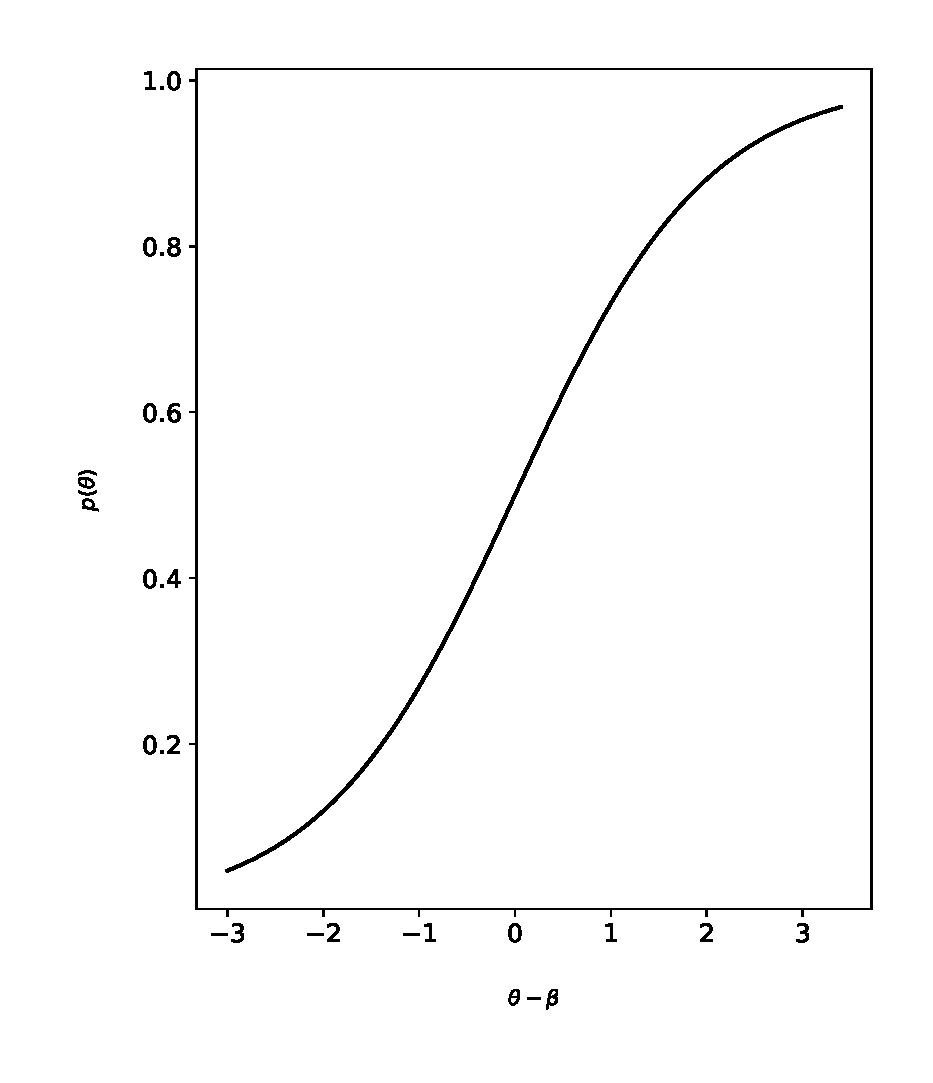
\includegraphics[width=.5\textwidth]{fig/irt.eps} 
   \caption{A probability curve in Item Response Theory.}
  \end{figure}
}



\frame{ \frametitle{Item Response Theory MLE}
  \begin{figure}[p!]
   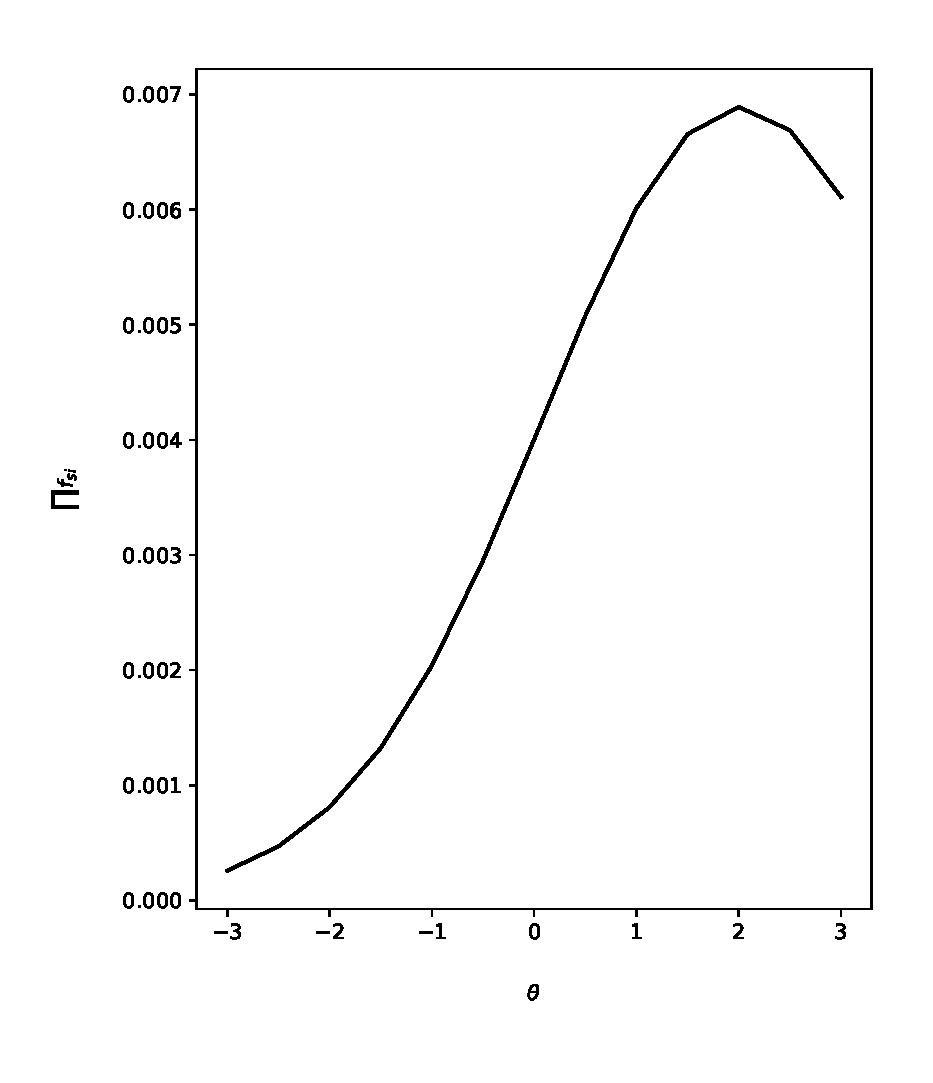
\includegraphics[width=.5\textwidth]{fig/mle.eps} 
   \caption{A maximum likelihood estimation with Item Response Theory.}
  \end{figure}
}



\frame{ \frametitle{Grades}
  \small
  \centering
  \begin{tabular}{||l|c|l||}
  \hline\hline
  Letter  & $\theta$  & Explanation \\\hline
  F  & -3.0   & unsatisfactory \\\hline
  D- & -2.5   &                \\
  D  & -2.0   & minimal        \\
  D+ & -1.5   &                \\\hline
  C- & -1.0   &                \\
  C  & -0.5   & acceptable     \\
  C+ & 0.0    &                \\\hline
  B- & 0.5    &                \\
  B  & 1.0    & good           \\
  B+ & 1.5    &                \\\hline
  A- & 2.0    &                \\
  A  & 2.5    & distinguished  \\
  A+ & 3.0    &                \\\hline\hline
  \end{tabular}
  \normalsize
}



\end{document}
